%% ============================================================
%%  STANDARD PREAMBLE (article, lecture notes)
%% ============================================================

% ---------- Document class and page layout ----------
\documentclass[11pt]{article}      % Basic document type, 11pt body text
\usepackage[margin=1in]{geometry}  % Sets page margins to 1 inch on all sides

% ---------- Paragraph style ----------
\usepackage{setspace}              % Lets you set the line spacing of the whole document
\setstretch{1.2}                   % Line spacing factor: 1.0 = single (default), 1.2 = slightly airy, 1.5 = very loose
\setlength{\parindent}{2em}        % First-line indent of each paragraph
\setlength{\parskip}{1\baselineskip} % Extra vertical gap between paragraphs

% ---------- Math ----------
\usepackage{amsmath,amssymb}       % Core math: align, cases, \text{}, plus extra symbols (\mathbb, \hbar, ...)

% ---------- Colors and boxes ----------
\usepackage{xcolor}                % Lets you use colors (\textcolor{red}{...})
\usepackage{mdframed}              % Boxes around text that can break across pages (theorems, key results)

% ---------- Diagrams ----------
\usepackage{tikz-cd}               % Commutative diagrams / arrow diagrams (also loads tikz)
\usepackage{tikz}                  % General-purpose drawing: lines, shapes, plots
\usetikzlibrary{arrows.meta, positioning, decorations.pathreplacing} % arrows.meta: more arrow tip styles; positioning: place nodes "right=of A"; decorations.pathreplacing: curly braces for labels

% ---------- Text layout ----------
\usepackage{multicol}              % Multi-column text (\begin{multicols}{2} ... \end{multicols})
\usepackage{indentfirst}           % Indents the first paragraph after a heading (article class skips it by default)

% ---------- Hyperlinks ----------
\usepackage[hidelinks]{hyperref}   % Clickable TOC, \ref, \eqref, \cite; hidelinks = no colored text or boxes

% ---------- Equation numbering ----------
\numberwithin{equation}{section}   % Equation counter resets in each section and displays as section.equation, e.g. (2.3)

% ---------- Title block ----------
\title{Quantum Mechanics Review}
\author{Duy M. Dao}
\date{\today}                      % Compile date; replace with a fixed date if you prefer

\begin{document}
\maketitle                         % Prints title, author, date
%\tableofcontents                   % Clickable table of contents

\newpage

\section{Representation of a Quantum State}

\paragraph{The state is an abstract vector.} A quantum state $|\Phi\rangle$ of a system with Hamiltonian $\hat H$ is an abstract \textcolor{blue}{state vector}. The state vector belongs to a \textcolor{blue}{Hilbert space} $\mathcal{H}$, which is a complex vector space with an inner product. The state vector, therefore, obeys the rules of an ordinary vector. For any states $|\Phi\rangle$, $|\Psi\rangle$, $|\chi\rangle$ in $\mathcal{H}$ and any complex numbers $a$, $b$, the rules are
\begin{itemize}
    \item closure under addition, so any superposition $|\Phi\rangle + |\Psi\rangle$ is also a state in $\mathcal{H}$;
    \item commutative and associative addition, so $|\Phi\rangle + |\Psi\rangle = |\Psi\rangle + |\Phi\rangle$ and $(|\Phi\rangle + |\Psi\rangle) + |\chi\rangle = |\Phi\rangle + (|\Psi\rangle + |\chi\rangle)$;
    \item a zero vector $0$ with $|\Phi\rangle + 0 = |\Phi\rangle$, and an inverse $-|\Phi\rangle$ with $|\Phi\rangle + (-|\Phi\rangle) = 0$;
    \item closure under multiplication by any complex number, so $a|\Phi\rangle$ is also in $\mathcal{H}$;
    \item distributive and associative multiplication, so $a(|\Phi\rangle + |\Psi\rangle) = a|\Phi\rangle + a|\Psi\rangle$, $(a+b)|\Phi\rangle = a|\Phi\rangle + b|\Phi\rangle$ and $a(b|\Phi\rangle) = (ab)|\Phi\rangle$, with $1|\Phi\rangle = |\Phi\rangle$;
    \item an inner product $\langle\Psi|\Phi\rangle$, which is a complex number that is linear in $|\Phi\rangle$, satisfies $\langle\Psi|\Phi\rangle = \langle\Phi|\Psi\rangle^*$, and gives $\langle\Phi|\Phi\rangle \geq 0$ with equality only for the zero vector.
\end{itemize}
The state itself is not measured. Measurements give values of the \textcolor{blue}{observables}, such as momentum, energy and angular momentum, and the state determines the probability of each value.

\paragraph{The wavefunction is the state written in the position basis.} The familiar wavefunction $\Phi(x)$ is not the state itself. The wavefunction is the \textcolor{blue}{position representation} of the state vector, and the other observables, such as momentum, can be calculated from it. Each value $\Phi(x)$ is the component of $|\Phi\rangle$ along the \textcolor{blue}{position eigenstate} $|x\rangle$:
\begin{equation}
    \boxed{\Phi(x) = \langle x | \Phi \rangle}
\end{equation}
The wavefunction is, therefore, a \textcolor{blue}{probability amplitude}. The value $\Phi(x)$ is a complex number, and the squared modulus $|\Phi(x)|^2$ is the probability density. The amplitude is the square root of the probability density, up to a phase $\theta(x)$:
\begin{equation*}
    \Phi(x) = \sqrt{|\Phi(x)|^2}\; e^{i\theta(x)}
\end{equation*}

\paragraph{The wavefunction is an infinite array of components.} The wavefunction can be viewed as an infinite array with one complex number for each position $x$. The array works like the list of components of an ordinary vector, with the position $x$ in the role of the index $i$. A three-dimensional vector is rebuilt from the components as
\begin{equation*}
    |v\rangle = \sum_i v_i\, |e_i\rangle, \qquad v_i = \langle e_i | v \rangle
\end{equation*}
The state vector is rebuilt in the same way. The \textcolor{blue}{completeness relation} of the position eigenbasis is
\begin{equation*}
    \int dx'\, |x'\rangle\langle x'| = \mathbb{I}
\end{equation*}
Inserting the completeness relation in front of $|\Phi\rangle$ gives
\begin{equation*}
    |\Phi\rangle = \int dx'\, |x'\rangle\langle x' | \Phi \rangle
\end{equation*}
\begin{equation}
    \boxed{|\Phi\rangle = \int dx'\, \Phi(x')\, |x'\rangle}
\end{equation}

\paragraph{Discretizing the wavefunction turns the integral into a sum over array entries.} The array picture becomes concrete when the position axis is cut into points $x_i = i\,\Delta x$ with a small spacing $\Delta x$. Figure~\ref{fig:array} uses the wavefunction $\Phi(x) = \sqrt{2/\pi}\,\sin x$ on the interval $0 \leq x \leq \pi$, which is the ground state of an infinite square well of width $\pi$. Each point $x_i$ stores one number $\Phi(x_i)$, and the list of these numbers is a column vector with $N$ entries. The integral over $x'$ in the expansion of $|\Phi\rangle$ is the limit of a sum over these entries:
\begin{equation*}
    |\Phi\rangle = \int dx'\, \Phi(x')\, |x'\rangle = \lim_{\Delta x \to 0}\, \sum_{i=1}^{N} \Delta x\, \Phi(x_i)\, |x_i\rangle
\end{equation*}
The number of entries $N = \pi/\Delta x$ grows without limit as $\Delta x \to 0$. The finite column vector, therefore, becomes the continuous function $\Phi(x)$ with one entry for every real number $x$.

\begin{figure}[h]
    \centering
    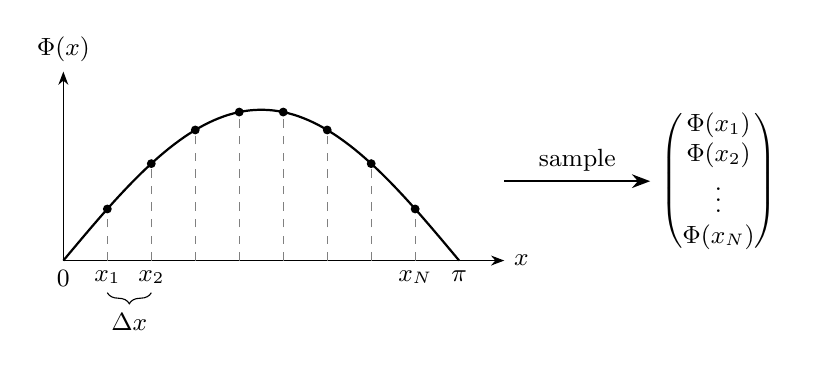
\begin{tikzpicture}[>=Stealth, x=1.6cm, y=2.4cm, font=\small]
        % axes
        \draw[->] (0,0) -- (3.5,0) node[right] {$x$};
        \draw[->] (0,0) -- (0,1.0) node[above] {$\Phi(x)$};
        \node[below] at (0,0) {$0$};
        \node[below] at (pi,0) {$\pi$};
        % continuous wavefunction
        \draw[thick, domain=0:pi, samples=80] plot (\x, {0.798*sin(\x r)});
        % sampled points x_1 ... x_N
        \foreach \i in {1,...,8} {
            \pgfmathsetmacro{\xi}{\i*pi/9}
            \pgfmathsetmacro{\yi}{0.798*sin(\xi r)}
            \draw[dashed, gray] (\xi,0) -- (\xi,\yi);
            \fill (\xi,\yi) circle (1.6pt);
        }
        \node[below] at ({pi/9},0) {$x_1$};
        \node[below] at ({2*pi/9},0) {$x_2$};
        \node[below] at ({8*pi/9},0) {$x_N$};
        % spacing between neighboring points
        \draw[decorate, decoration={brace, amplitude=4pt, mirror}] ({pi/9},-0.17) -- ({2*pi/9},-0.17) node[midway, below=4pt] {$\Delta x$};
        % array of sampled values
        \node (array) at (5.2,0.42) {$\begin{pmatrix} \Phi(x_1) \\ \Phi(x_2) \\ \vdots \\ \Phi(x_N) \end{pmatrix}$};
        \draw[->, thick] (3.5,0.42) -- (array.west) node[midway, above] {sample};
    \end{tikzpicture}
    \caption{Wavefunction $\Phi(x) = \sqrt{2/\pi}\,\sin x$ sampled at $N$ points with spacing $\Delta x$. The sampled values form a column vector with $N$ entries. The column vector becomes the continuous function for $\Delta x \to 0$ and $N \to \infty$.}
    \label{fig:array}
\end{figure}

\paragraph{The primed variable labels the basis and the unprimed variable is the evaluation point.} The two position variables have different roles. The primed variable $x'$ is a placeholder that runs over every position eigenstate $|x'\rangle$ in the integral, in the same way that the summation index $i$ runs over every basis vector $|e_i\rangle$. Renaming $x'$ does not change the expansion. The unprimed variable $x$ is the single position at which the wavefunction is evaluated, so $x$ plays the role of a fixed component index $j$. For the ordinary vector, the fixed component follows from the orthonormality $\langle e_j | e_i \rangle = \delta_{ji}$:
\begin{align*}
    \langle e_j | v \rangle &= \sum_i v_i\, \langle e_j | e_i \rangle \\
    &= \sum_i v_i\, \delta_{ji} \\
    &= v_j
\end{align*}
The position eigenstates satisfy the continuous version of this orthonormality, $\langle x | x' \rangle = \delta(x - x')$. The projection of the expansion back onto $\langle x|$, therefore, recovers one entry of the array:
\begin{align*}
    \langle x | \Phi \rangle &= \int dx'\, \Phi(x')\, \langle x | x' \rangle \\
    &= \int dx'\, \Phi(x')\, \delta(x - x') \\
    &= \Phi(x)
\end{align*}
The delta function selects the entry at $x' = x$ in the same way that the Kronecker delta $\delta_{ji}$ selects the component $v_j$. The position eigenstates are not normalizable, because $\langle x | x \rangle = \delta(0)$ diverges. Strictly, $|x\rangle$ lies outside $\mathcal{H}$, and the rigorous framework is the \textcolor{blue}{rigged Hilbert space}. The position eigenstates are still used as a basis, because every physical state is a normalizable superposition of them.

\paragraph{A function is also an abstract vector.} The whole function $\Phi$, rather than a single value $\Phi(x)$, is itself a vector for the same reason as $|\Phi\rangle$. The \textcolor{blue}{square-integrable functions}, with $\int |\Phi(x)|^2\, dx$ finite, form the vector space $L^2$. The sum of two square-integrable functions is square-integrable, a complex multiple of a square-integrable function is square-integrable, and the zero function is the zero vector. The functions, therefore, obey every rule of the list above. The inner product of $|\Psi\rangle$ and $|\Phi\rangle$ follows from the completeness relation:
\begin{align*}
    \langle \Psi | \Phi \rangle &= \int dx\, \langle \Psi | x \rangle \langle x | \Phi \rangle \\
    &= \int dx\, \langle x | \Psi \rangle^* \langle x | \Phi \rangle
\end{align*}
\begin{equation}
    \boxed{\langle \Psi | \Phi \rangle = \int dx\, \Psi^*(x)\, \Phi(x)}
\end{equation}
The map from $|\Phi\rangle$ to $\Phi(x)$ keeps sums, complex multiples and inner products unchanged. The Hilbert space $\mathcal{H}$ and the function space $L^2$ are, therefore, two descriptions of the same vectors. The state vector is the basis-free description, and the wavefunction is the description in the position basis.

\end{document}
